% =====================================================================
% Diploma thesis -- HTL Donaustadt, Department of Information Technology
%
% Build:  make          (or: latexmk -pdf diplomarbeit.tex)
%
% Class options:
%   deutsch (default) | englisch
%   ieee (default)    | harvard
%   lato (default)    | inter | carlito | aptos
%   entwurf           -- ENTWURF (draft) watermark on every page
% =====================================================================
\documentclass[deutsch,ieee,lato]{htldon}
\usepackage{amsmath}

\addbibresource{references.bib}

% =====================================================================
% Everything about your thesis in ONE place.
% This is the only file you have to fill in to get started.
% =====================================================================

\titel{VerTeX - Automatische Videoanalyse und Spielstatistiken im Fußball }

% Short title: appears on the left of every page header. Keep it short!
\kurztitel{VerTeX MatchAnalytics}

% Optional project logo on the title page. Delete the line if you have none.
\projektlogo{images/Logo.jpeg}


% Project team -- the order here is the order on the title page.
% Syntax: \teammitglied[short form for the page header]{SURNAME}{Given name}
% The short form is derived automatically ("M. Musterfrau"). Only pass it
% yourself if the given name starts with a special character (Ö, Č, ...).
\teammitglied{AKPINAR}{Emre}
\teammitglied{ISHAK}{Mohamed}
\teammitglied{RAHAL}{Jobanpreet Singh}

% Supervisors -- the optional argument is the label on the title page.
\betreuung[Betreuerin]{Ing. Peter ÖTTL, MSc}
\betreuung[Betreuer]{ Alessa STRIA, BSc}

\schuljahr{2026/27}
\abteilung{Informationstechnologie}
\klasse{5AHITN}

\ort{Wien}

% Date under the declaration of authorship. Left out, it is the build date --
% which is what you want while writing, because the printout you sign carries
% the day you printed it. Pin it only if the school asks for a fixed date:
% \abgabedatum{1. April 2027}


\begin{document}

% --- Front matter (no page numbers, not in the table of contents) -----
\titelblatt
\eigenstaendigkeitserklaerung
% =====================================================================
% Problem statement -- carries over the content of the approved topic
% proposal. Please do not change the structure.
% =====================================================================
\vorspannkapitel{Problemstellung}
\abschnittsautor{\alleautoren}

\vorspannabschnitt{Ausgangslage}

Automatisierte Spielanalyse (Laufdistanzen, Positionsdaten, Ereigniserkennung) ist im Profifußball Standard, 
für Amateur- und Jugendvereine aber kaum zugänglich: bestehende 
Systeme sind teuer, an Spezialhardware gebunden und geschlossen. 
Vereine filmen zwar oft mit einfachen Kameras, können die 
Aufnahmen aber nicht automatisiert auswerten.

\vorspannabschnitt{Untersuchungsanliegen der individuellen Themenstellungen}

\vorspannunterpunkt{1) Teilbereich A Akpinar }
Welche Messabweichungen und Genauigkeitsgrenzen entstehen bei der 
2D-Homographie ohne echte 3D-Tiefsensoren

\vorspannunterpunkt{2) Teilbereich B Ishak}
Wie verändert sich die Detektionsgenauigkeit bei Spielerverdeckung
durch spezifisches Fine-Tuning im vergleich zu Standard-Basismodellen?

\vorspannunterpunkt{3) Teilbereich C Rahal}
Wie muss eine Systemarchitektur ausgelegt sein, 
um hochfrequente Tracking-Rohdaten mit minimaler Latenz 
abzufragen und für Laien intuitiv darzustellen?
\vorspannabschnitt{Zielsetzung}

Am Ende der Arbeit liegt ein funktionsfähiger Software-Prototyp 
vor, der Fußballspiele über ein Zwei-Kamera-Panoramasystem 
erfasst, Spieler mittels Computer Vision trackt und deren 
Bewegungsdaten als reale 2D-Spielfeldkoordinaten in einem 
interaktiven Web-Dashboard visualisiert.

\vorspannabschnitt{Geplantes Ergebnis der individuellen Themenstellungen}

\vorspannunterpunkt{1) Teilbereich A Akpinar}
Artefakt:

Eine Software-Pipeline, die das Video-Stitching beider Kameras 
durchführt, Tracking-IDs vergibt und die Pixelkoordinaten über 
eine kalibrierte Homographie-Matrix in ein reales Koordinatensystem
(in Metern) umrechnet.

Messbarkeit:

Toleranz- und Fehleranalyse: Abweichung der berechneten Distanzen
gegenüber real vermessenen Referenzstrecken auf dem Platz 
(z. B. prozentualer Messfehler bei 16-Meter-Raum, Mittellinie) 
sowie Stabilität des Trackings (Anzahl der ID-Switches).

\vorspannunterpunkt{2) Teilbereich B Ishak}
Artefakt:

Ein exportiertes, lauffähiges Modell 
(.pt / .yaml), die zugehörige Trainings- und Inferenz-Pipeline 
sowie der vorbereitete, annotierte Validierungsdatensatz. 

Messbarkeit: 

Quantitative Evaluierungsmetriken: $mAP_{50}$, $mAP_{50-95}$, 
Precision, Recall und Inferenzzeit (FPS / Latenz in ms) bei 
Szenarien mit Verdeckung im Vergleich zum ungetunten Basismodell.

\vorspannunterpunkt{3) Teilbereich C Rahal}
Artefakt:

Ein lauffähiges Softwaresystem bestehend aus 
relationalem/zeitreihenbasiertem Datenbankschema, REST- bzw. 
WebSocket-API zur Datenabfrage und einem interaktiven Web-Frontend.
Wie wird es überprüft 

Messbarkeit:

Funktionale Abnahmekriterien: End-to-End-Test 
Import von Trackingdaten $\rightarrow$ korrekte 
visuelle Ausgabe auf dem 2D-Taktikfeld, Rendern von Heatmaps) 
und Performance-Benchmarks (z. B. API-Antwortzeiten unter Last).

\vorspannabschnitt{Meilensteine}

% Deliberately not a table float: the milestones belong directly under the
% heading, not somewhere else in the document.
\begin{tabular}{@{}p{0.68\linewidth}p{0.24\linewidth}@{}}
    \toprule
    \bfseries Meilenstein & \bfseries Datum \\
    \midrule
    Analyse der Ausgangslage und Anforderungen & 30.09.2026 \\
    Erstellung der Konzepte                    & 31.10.2026 \\
    Implementierung der Systemkomponenten      & 30.11.2026 \\
    Test der Systemkomponenten                 & 15.01.2027 \\
    Integration des Gesamtsystems              & 15.02.2027 \\
    Verfassen der Dokumentation                & 15.03.2027 \\
  Abgabe der Diplomarbeit                    & 01.04.2027 \\
  \bottomrule
\end{tabular}

% =====================================================================
% Kurzfassung (German), Abstract (English), acknowledgements
% Rule of thumb: half a page to a page each, no sources, no figures.
% =====================================================================

\kurzfassung{%
Die Kurzfassung beschreibt in wenigen Absätzen, worum es in der Arbeit geht:
Ausgangsproblem, gewählter Lösungsansatz, umgesetztes Ergebnis und der Nutzen
für die Anwenderinnen und Anwender. Sie muss ohne den Rest der Arbeit
verständlich sein.

Der zweite Absatz beschreibt üblicherweise die technische Umsetzung auf
Überblicksebene: welche Komponenten entstanden sind und wie sie zusammenspielen.

Der letzte Absatz fasst das Ergebnis zusammen und benennt den erzielten
Mehrwert.

Die Spielanalyse im Fussball (Laufdistanzen, Positionsdaten und taktischen
Auswertungen) kostet oft Geld und viel Hardware. Kleine Vereine können sich diese Funktion oft nicht leisten. Das Diplomprojekt
VerTex setzt hier an. Es ist ein System das aus Videoaufnahmen des Spielfelds Bewegungs- und Spielstatistiken
gewinnt und diese Trainerinnen und Trainern ohne technisches Vorwissen
zugänglich macht.

Das Spielfeld wird mit einem synchronisierten Zwei-Kamera-Setup erfasst und zu
einem Panorama zusammengefügt. Ein Computer-Vision-Modell erkennt Spieler und Ball und verfolgt sie über die ganze Spiellänge. 
Mittels einer Homogprahie werden die Bildkoordinaten in Spielfeldkoordinaten umgerechnet. 
Die Bewegungsdaten werden über eine API in einer Datenbank gespeichert. 
Aus den Daten werden Laufwege, Distanzen und Teamstatistiken berechnet. 
Eine Web-Applikation greift über die API auf die Daten zu und stellt sie interaktiv dar.

Als Ergebnis soll eine interaktive Web-Applikation zur Verfügung gestellt werden,
die die Auswertung von Heatmaps und Teamstatistiken visuell darstellt. 
Weiters, soll ein fine-getuntes Computer-Vision-Modell für fußballspezifische Objekterkennung entwickelt werden. 




}

\abstracttext{%
The abstract is the English translation of the Kurzfassung. It covers the same
content in the same structure: the initial problem, the chosen approach, the
implemented result, and the benefit for its users.

The second paragraph outlines the technical realisation at an overview level:
which components were built and how they interact.

The final paragraph summarises the outcome and states the value it creates.

Match analysis in football (running distances, position data and tactical
evaluations) often requires a lot of money and hardware. Small clubs frequently
cannot afford this functionality. The diploma project VerTex addresses this
problem. It is a system that derives movement and match statistics from video
recordings of the pitch and makes them accessible to coaches without any
technical background.

The pitch is captured with a synchronised two-camera setup, and the images are
stitched into a panorama. A computer vision model detects players and the ball
and tracks them over the entire duration of the match. Using a homography, the
image coordinates are converted into pitch coordinates. The movement data is
stored in a database via an API. Running paths, distances and team statistics
are calculated from this data. A web application accesses the data through the
API and presents it interactively.

As a result, an interactive web application is to be provided that visualises
the evaluation of heatmaps and team statistics. Furthermore, a fine-tuned
computer vision model for football-specific object detection is to be
developed.
}

\danksagung{%
An dieser Stelle bedanken wir uns bei allen, die uns während der Erstellung
dieser Diplomarbeit unterstützt haben.

Unser besonderer Dank gilt unseren Betreuerinnen und Betreuern für die
fachliche Unterstützung und die investierte Zeit.
}


\inhaltsverzeichnis

% --- Main part -------------------------------------------------------
\chapter{Einleitung}
% \abschnittsautor controls who appears on the right of the page header. It
% works per section too, not just per chapter -- call it again after any
% \section that a different team member wrote. ALWAYS call it directly after
% the heading, otherwise it takes effect one page too early.
\abschnittsautor{\alleautoren}

\section{Motivation}

Die Einleitung führt in das Thema ein: Warum ist die Aufgabenstellung
relevant, in welchem Umfeld tritt sie auf, und was passiert, wenn sie
ungelöst bleibt? Belege gehören hier bereits mit Quellenangabe
dazu~\cite{beispiel-buch}.

Die datengestütze Analyse von Spiel- und Trainingsdaten bildet im mordernen
Profifußball das Fundament für taktische Entscheidungen, Leistungsdiagnostik
und Verletzungspräventation~\cite{}

\section{Zielsetzung}

Beschreibt das Ziel so, dass am Ende der Arbeit überprüfbar ist, ob ihr es
erreicht habt. Trennt dabei funktionale von nichtfunktionalen Anforderungen.

Ein Absatz wird durch eine Leerzeile im Quelltext erzeugt. Einen Zeilenumbruch
innerhalb eines Absatzes erzwingt ihr mit \verb|\\| -- braucht ihr aber fast nie.

\input{content/21-project-planning}
\chapter{Technische Grundlagen}
\abschnittsautor{M. Musterfrau}

Hier steht alles, was zum Verständnis der praktischen Umsetzung nötig ist --
und nur das. Jede Technologie, die ihr später verwendet, wird hier einmal
erklärt und belegt.

\section{Teilbereich A}

Beim ersten Auftreten schreibt ihr eine Abkürzung aus: \ac{API}. Danach
genügt die Kurzform: \ac{API}. Alle Abkürzungen sammelt ihr in
\texttt{diplomarbeit.tex} im Abkürzungsverzeichnis.

\subsection{Ein Unterabschnitt}

Zitiert wird im IEEE-Stil mit einer Nummer in eckigen
Klammern~\cite{beispiel-artikel}. Mehrere Quellen auf einmal gehen
auch~\cite{beispiel-buch,beispiel-online}.

\subsubsection{Eine Ebene tiefer}

Die vierte Ebene könnt ihr verwenden, aber sparsam. Sie wird nummeriert,
steht aber nicht mehr im Inhaltsverzeichnis. Tiefer gliedert ihr nicht.

\section{Teilbereich B}

Erklärt Technologien in eurer eigenen Formulierung. Wörtlich übernommene
Passagen gehören in Anführungszeichen und mit Seitenangabe belegt, sonst gilt
das als Plagiat.

\section{Computer Vision und Objekterkennung}
\abschnittsautor{M. Ishak}

Die automatisierte Erfassung von Fußballspielern auf einem Spielfeld erfordert robuste Algorithmen aus dem 
Bereich der \ac{CV}. In diesem Abschnitt werden die technologischen Grundlagen der Bildverarbeitung und der 
darauf aufbauenden Objekterkennung erläutert.

\subsection{Architektur von Convolutional Neural Networks}

Ein \ac{CNN} ist eine spezielle Form von künstlichen neuronalen Netzen, die primär für die Verarbeitung von 
Bild- und Audiodaten eingesetzt wird. Im Gegensatz zu klassischen \textit{Fully Connected Networks} bewahren
\acp{CNN} die räumliche Struktur von Bilddaten und arbeiten mit einer deutlich reduzierten Anzahl an 
Parametern, was sie recheneffizienter und robuster macht~\cite{goodfellow2016deep}.

Das Kernkonzept eines \ac{CNN} ist die Faltungsschicht (Convolutional Layer). Hierbei gleiten kleine Matrizen, 
sogenannte Filter oder Kernel, schrittweise über das Eingabebild und berechnen das Skalarprodukt zwischen 
den Filtergewichten und den Bildpixeln. In den frühen Schichten des Netzwerkes lernen diese Filter einfache 
visuelle Kanten, Ecken oder Farbkontraste. In tieferen Schichten setzen sich diese einfachen Merkmale zu 
komplexeren Mustern wie spezifischen Texturen oder Objektteilen zusammen~\cite{goodfellow2016deep}. Das 
Ergebnis dieser Faltungsoperationen sind sogenannte \textit{Feature Maps} (Merkmalskarten).

Um die räumliche Auflösung der Feature Maps zu reduzieren und gleichzeitig die wichtigsten Merkmale zu 
erhalten, kommen Pooling-Schichten (z.\,B.\ Max-Pooling) zum Einsatz. Diese fassen benachbarte Pixel 
zusammen und leiten nur den dominantesten Wert weiter. Dies senkt nicht nur den Rechenaufwand signifikant, 
sondern sorgt auch für eine Translationsinvarianz~-- das Netzwerk erkennt ein gelerntes Muster unabhängig 
von dessen exakter Position im Bild.

Nach mehreren Convolutional- und Pooling-Schichten wird die resultierende mehrdimensionale Matrix 
abgeflacht (Flattening) und an eine oder mehrere \textit{Fully Connected Layers} 
(vollständig verbundene Schichten) übergeben. Diese fungieren als Klassifikator: Sie wichten die 
extrahierten, hochkomplexen Merkmale und berechnen am Ende Wahrscheinlichkeiten für die gesuchten Klassen 
(beispielsweise „Fußballspieler“, „Schiedsrichter“ oder „Ball“). Der gesamte schematische Ablauf von der 
Merkmalsextraktion bis zur Klassifikation ist in Abb.~\ref{abb:cnn-architektur} dargestellt.

\begin{figure}[htbp]
    \centering
    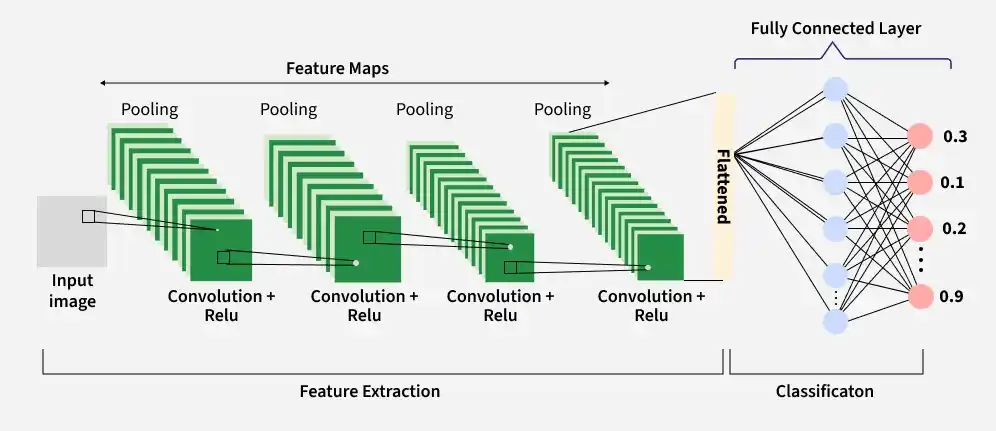
\includegraphics[width=0.9\linewidth]{images/working_of_cnn_ishak.png}
    \caption{Schematischer Aufbau eines Convolutional Neural Networks zur Bildklassifikation~\cite{gfg-cnn}.}\label{abb:cnn-architektur}
\end{figure}

\subsection{You Only Look Once (YOLO)}

Für die Objekterkennung in Echtzeit hat sich in den letzten Jahren die Modellarchitektur \ac{YOLO} als 
De-facto-Standard etabliert. Im Gegensatz zu zweistufigen Detektoren (wie etwa Faster R-CNN), die zuerst 
potenziell relevante Bildregionen vorschlagen und diese anschließend klassifizieren, formuliert \ac{YOLO} die 
Objekterkennung als ein einziges Regressionsproblem~\cite{redmon2016you}. Das gesamte Bild wird in einem 
einzigen Vorwärtsdurchlauf (Single-Pass) analysiert, um Bounding Boxes und Klassenzugehörigkeiten simultan 
vorherzusagen. Dies führt zu einer massiven Steigerung der Inferenzgeschwindigkeit.

Moderne \ac{YOLO}-Architekturen, wie das von Ultralytics entwickelte YOLOv8, bestehen grundlegend aus drei 
Hauptkomponenten: dem \textit{Backbone}, dem \textit{Neck} und dem \textit{Head}~\cite{ultralytics2023yolov8}. 
Das Backbone (basierend auf einem modifizierten CSPDarknet mit C2f-Modulen) dient als effizienter 
Feature-Extraktor. Der Neck (kombiniert aus einem Feature Pyramid Network und einem Path Aggregation Network) 
führt Merkmale aus verschiedenen Netzwerktiefen zusammen. Dies ist essenziell, um Objekte in stark 
unterschiedlichen Skalierungen zu erkennen~-- ein entscheidender Faktor im Fußball, wo Spieler in 
Kameranähe groß und auf der gegenüberliegenden Spielfeldseite sehr klein abgebildet werden. Der Head 
schlussendlich ist entkoppelt (\textit{Decoupled Head}) und arbeitet ankerfrei (\textit{Anchor-Free}): Er 
gibt auf zwei getrennten Pfaden separat die Wahrscheinlichkeiten für die Objektklassen sowie die genauen 
Koordinaten der Bounding Boxes aus.

Für die automatisierte Videoanalyse im Fußball ist YOLOv8 prädestiniert, da die hohe Inferenzgeschwindigkeit 
ein durchgehendes Frame-by-Frame-Tracking ermöglicht. Durch die Verarbeitung von hochauflösenden 
Eingabebildern (z.\,B.\ 1280 Pixel) lassen sich auch auf weite Distanzen zuverlässige Detektionen erzielen.

\subsection{Herausforderungen bei Verdeckung (Occlusion)}

Eine der größten Herausforderungen bei der optischen Verfolgung von Spielern im Fußball ist die sogenannte 
Verdeckung (Occlusion). Bei Zweikämpfen oder Standardsituationen, wie etwa einem Eckball, stehen Spieler 
dicht gedrängt und verdecken sich gegenseitig teilweise oder vollständig. Standard-Objekterkennungsmodelle 
stoßen hierbei systembedingt an ihre Grenzen.

Das Hauptproblem liegt im Post-Processing-Algorithmus der Modelle, der \ac{NMS}. \ac{YOLO} generiert für 
dasselbe Objekt oft mehrere leicht verschobene Bounding Boxes. Um diese zu bereinigen, berechnet die 
\ac{NMS} den \ac{IoU}-Wert~-- das Verhältnis der Schnittfläche zur Vereinigungsfläche zweier 
Boxen $A$ und $B$:
\begin{equation}
    \text{IoU}(A, B) = \frac{|A \cap B|}{|A \cup B|}
\end{equation}
Überschreitet dieser Wert einen definierten Schwellenwert (z.\,B.\ $0{,}45$), geht der Algorithmus davon aus, 
dass beide Boxen dasselbe Objekt markieren, und löscht die Box mit der geringeren \textit{Confidence} 
(Konfidenz)~\cite{bodla2017soft}. Stehen jedoch zwei Fußballspieler im Zweikampf dicht hintereinander, 
überschneiden sich ihre echten Bounding Boxes extrem stark. Standard-\ac{NMS} bewertet den teilweise 
verdeckten Spieler fälschlicherweise als redundante Detektion des vorderen Spielers und unterdrückt 
ihn komplett.

Um diese Problematik zu beheben, erfordert es spezialisierte Lösungsansätze. Einerseits muss durch gezieltes 
Fine-Tuning auf fußballspezifische Datensätze trainiert werden, die eine hohe Dichte an Spielerverdeckungen 
(Ground Truth) aufweisen, wie in Abb.~\ref{abb:occlusion-beispiel} exemplarisch dargestellt ist. 
Andererseits kommen spezifische Data-Augmentation-Methoden sowie angepasste \ac{IoU}-Schwellenwerte 
oder tolerantere Verfahren wie Soft-\ac{NMS}~\cite{bodla2017soft} zum Einsatz, um die Detektionsrate 
(Recall) bei starker Verdeckung signifikant zu steigern.

\begin{figure}[htbp]
    \centering
    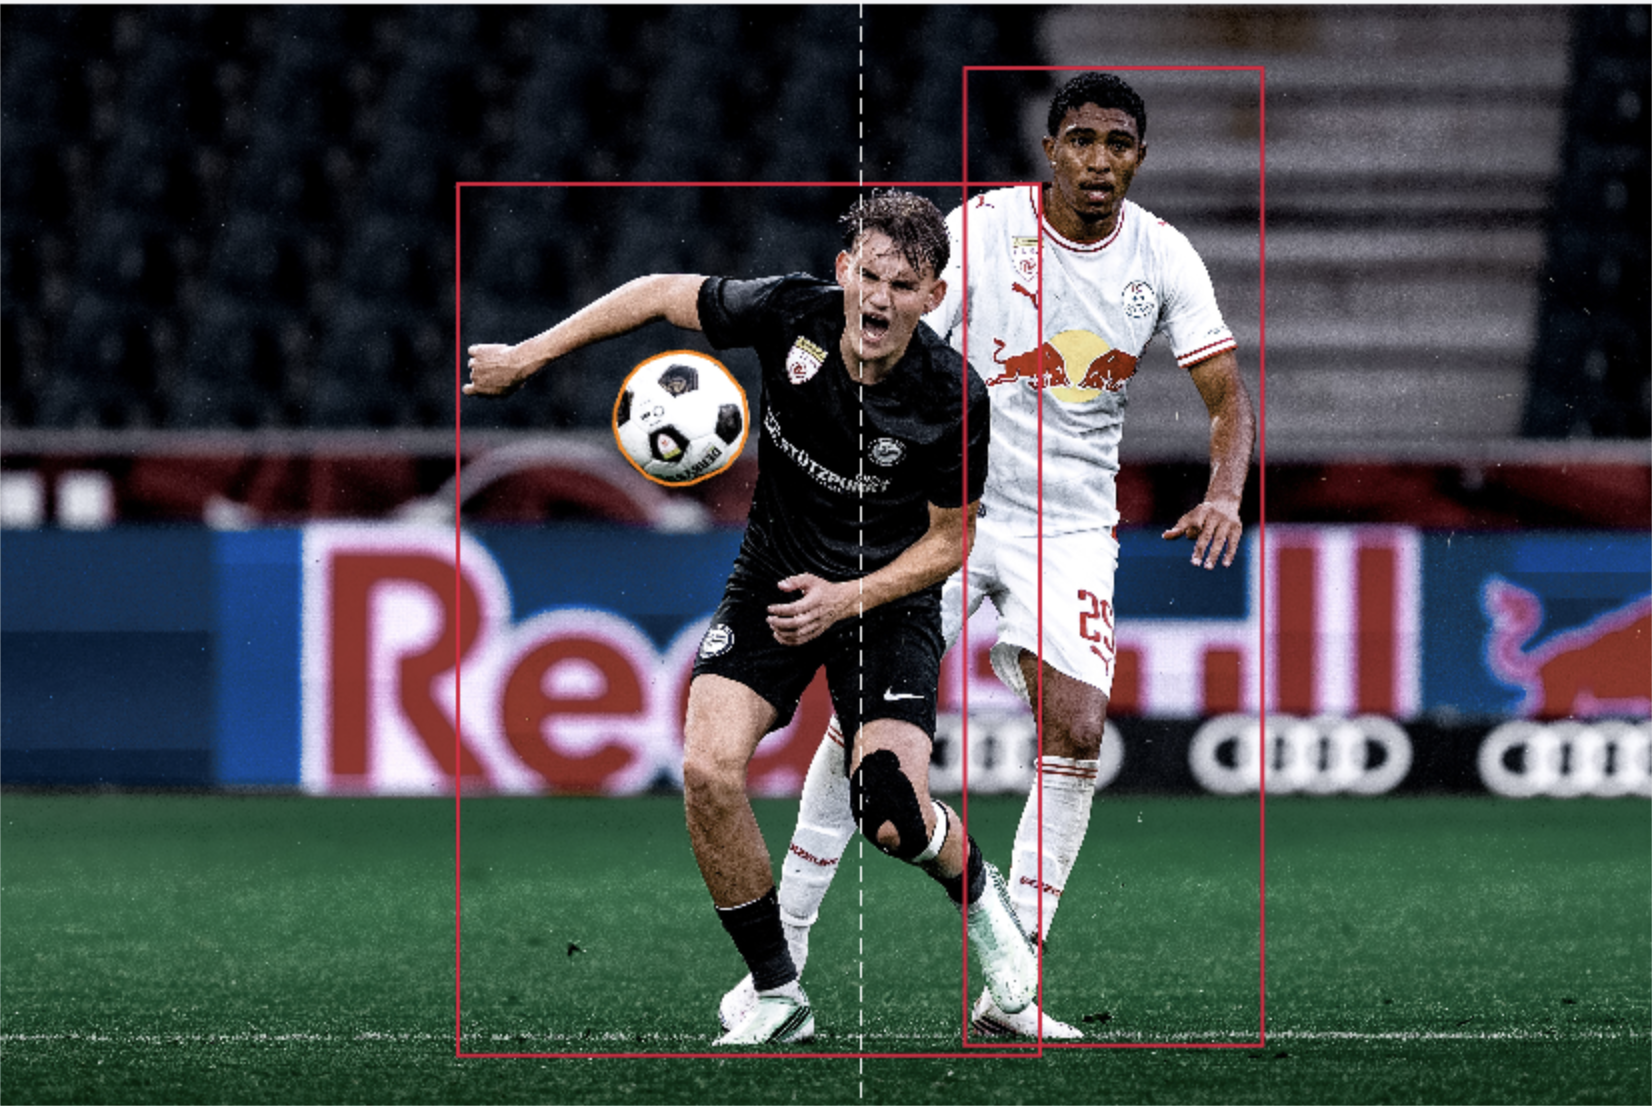
\includegraphics[width=0.75\linewidth]{images/roboflow_bounding_box_ishak.png}
    \caption{Beispiel einer starken Verdeckung (Occlusion) im Fußball. Der hintere Spieler wird trotz massiver Überlappung separat annotiert und detektiert (eigene Darstellung in Roboflow).}\label{abb:occlusion-beispiel}
\end{figure}

\subsection{Transfer Learning und Fine-Tuning}

Das Training eines tiefen neuronalen Netzes von Grund auf (Training from Scratch) erfordert 
hunderttausende annotierte Bilder sowie massive Rechenkapazitäten, um grundlegende Merkmale wie Kanten 
und einfache geometrische Formen zu erlernen. Um diese Ressourcenhürde zu umgehen, wird in der modernen 
Bildverarbeitung das Prinzip des \textit{Transfer Learning} (Wissenstransfer) angewandt~\cite{pan2009survey}.

Dabei wird ein Basismodell verwendet, das bereits auf einem enormen, generischen Datensatz~-- wie 
dem \ac{COCO}-Datensatz mit über 330.000 Bildern und 80 Objektklassen~-- vortrainiert wurde. Die 
unteren Schichten (Backbone) dieses Modells haben bereits die Fähigkeit zur generellen Merkmalsextraktion 
perfektioniert. Beim sogenannten \textit{Fine-Tuning} werden die Gewichte des Netzes mit einer reduzierten 
Lernrate auf einen neuen, spezifischen Zieldatensatz~-- in diesem Fall fußballspezifische Aufnahmen~-- 
nachtrainiert und angepasst. Dies ermöglicht es, das Modell mit einer verhältnismäßig kleinen Menge an 
domänenspezifischen Trainingsdaten (wenige tausend Bilder) hocheffizient auf die Zielklassen 
(Spieler, Tormann, Ball, Schiedsrichter) zu spezialisieren, während irrelevante Klassen des 
Ursprungsmodells verworfen werden.

\subsection{Evaluierungsmetriken der Objekterkennung}

Um die Leistungsfähigkeit und Genauigkeit eines Objekterkennungsmodells objektiv beurteilen zu können, 
werden standardisierte Metriken herangezogen~\cite{padilla2020survey}. Grundlage hierfür ist der 
bereits erwähnte \ac{IoU}-Wert. Ein Detektionsergebnis gilt als \textit{True Positive} (TP), wenn der 
\ac{IoU} zwischen der vorhergesagten Bounding Box und der tatsächlichen Ground-Truth-Box einen 
definierten Schwellenwert (meist $0{,}50$) überschreitet. Liegt der Wert darunter oder wird ein 
Hintergrundobjekt fälschlicherweise markiert, resultiert ein \textit{False Positive} (FP). Wird ein 
reales Objekt vom Modell komplett übersehen, spricht man von einem \textit{False Negative} (FN).

Aus diesen Klassifikationen leiten sich die zwei fundamentalen Metriken ab:
\begin{itemize}
    \item \textbf{Precision (Genauigkeit):} Berechnet sich aus $\frac{TP}{TP + FP}$. Sie gibt an, wie viel Prozent der vom Modell gesetzten Bounding Boxes tatsächlich korrekte Objekte einkreisen. Eine hohe Precision bedeutet wenige Fehlalarme (z.\,B.\ wenn Werbebanden fälschlicherweise als Spieler erkannt werden).
    \item \textbf{Recall (Trefferquote):} Berechnet sich aus $\frac{TP}{TP + FN}$. Sie gibt an, wie viel Prozent der tatsächlich auf dem Bild vorhandenen Objekte vom Modell gefunden wurden. Im Kontext der Spielerverdeckung (Occlusion) ist der Recall die kritischste Metrik, da er aufzeigt, wie viele verdeckte Spieler fälschlicherweise übersehen wurden.
\end{itemize}

Um das Modell über verschiedene Konfidenz-Schwellenwerte hinweg bewerten zu können, wird die Fläche unter 
der Precision-Recall-Kurve berechnet, die sogenannte \textit{Average Precision} (AP). Der Mittelwert der 
AP über alle trainierten Klassen hinweg ergibt die \textit{mean Average Precision} (mAP). In aktuellen 
Evaluierungen wird häufig die Metrik \textbf{mAP@50--95} herangezogen. Hierbei wird die mAP über zehn 
verschiedene \ac{IoU}-Schwellenwerte (von $0{,}50$ bis $0{,}95$ in $0{,}05$-Schritten) 
gemittelt~\cite{padilla2020survey}. Ein hoher mAP@50--95-Wert garantiert nicht nur, dass das Objekt 
überhaupt gefunden wurde, sondern dass die Kanten der Bounding Box millimetergenau am Objekt anliegen~-- eine 
essenzielle Voraussetzung für die anschließende geometrische Homografie-Transformation in 
2D-Spielfeldkoordinaten.

\subsection{Verlustfunktionen (Loss-Architektur) in YOLOv8}

Während des Trainingsprozesses optimiert YOLOv8 seine Netzwerkgewichte durch die Minimierung einer 
zusammengesetzten Verlustfunktion (Loss Function). Da der Decoupled Head von YOLOv8 Klassifikation und 
Lokalisierung trennt, setzt sich der Gesamtverlust aus drei gewichteten Komponenten 
zusammen~\cite{ultralytics2023yolov8}:
\begin{equation}
    \mathcal{L}_{\text{total}} = \lambda_{\text{box}} \mathcal{L}_{\text{CIoU}} + \lambda_{\text{dfl}} \mathcal{L}_{\text{DFL}} + \lambda_{\text{cls}} \mathcal{L}_{\text{BCE}}
\end{equation}

Für die Klassifikation der vier Zielklassen kommt der \ac{BCE}-Verlust $\mathcal{L}_{\text{BCE}}$ zum Einsatz, 
der für jede Klasse unabhängig die Wahrscheinlichkeit berechnet. Für die räumliche Präzision der Bounding 
Boxes~-- welche für die Berechnung des Spieler-Fußpunktes entscheidend ist~-- kombiniert YOLOv8 zwei 
spezialisierte Lokalisierungsverluste:
\begin{itemize}
    \item \textbf{Complete IoU Loss ($\mathcal{L}_{\text{CIoU}}$):} Im Gegensatz zum einfachen \ac{IoU}-Verlust berücksichtigt der \ac{CIoU} zusätzlich den euklidischen Abstand zwischen den Mittelpunkten der vorhergesagten Box $b$ und der Ground-Truth-Box $b^{gt}$ sowie die Konsistenz des Seitenverhältnisses (Aspect Ratio) $v$~\cite{zheng2020distance}:
    \begin{equation}
        \mathcal{L}_{\text{CIoU}} = 1 - \text{IoU} + \frac{\rho^2(b, b^{gt})}{c^2} + \alpha v
    \end{equation}
    Hierbei bezeichnet $c$ die Diagonale des kleinsten umschließenden Rechtecks beider Boxen. Dadurch konvergiert das Modell deutlich schneller auf die exakte Körperform von stehenden oder laufenden Spielern.
    \item \textbf{Distribution Focal Loss ($\mathcal{L}_{\text{DFL}}$):} Bei starker Verdeckung (Occlusion) im Strafraum sind die Kanten einer Bounding Box oft mehrdeutig, da Körperteile durch Gegenspieler verdeckt werden. Anstatt die Box-Koordinaten als starre Einzelwerte (Dirac-Delta-Verteilung) vorherzusagen, modelliert der \ac{DFL} die Position jeder Box-Kante als diskrete Wahrscheinlichkeitsverteilung~\cite{li2020generalized}. Dies erlaubt es dem Netzwerk, Unsicherheiten an verdeckten Körperkanten mathematisch abzubilden und dennoch scharfe Begrenzungsboxen zu schätzen.
\end{itemize}

\subsection{Mathematische Grundlagen der Data Augmentation}

Um eine Überanpassung (Overfitting) des Modells an die Trainingsdaten zu verhindern und die 
Generalisierungsfähigkeit bei schwierigen Licht- und Verdeckungsverhältnissen zu erhöhen, wird 
während des Fine-Tunings eine dynamische Datenaugmentierung (Online Data Augmentation) durchgeführt. 
Die Trainingsbilder werden dabei in jeder Epoche vor dem Durchlauf durch das Netz zufällig transformiert. 
Tab.~\ref{tab:augmentation-methoden} fasst die für die Fußballanalyse relevanten Augmentierungsverfahren 
und deren spezifischen Nutzen zusammen.

\begin{table}[htbp]
    \centering
    \caption{Eingesetzte Data-Augmentation-Verfahren zur Steigerung der Modellrobustheit}\label{tab:augmentation-methoden}
    \begin{tabularx}{\linewidth}{llX}
        \tabkopf{}
        Verfahren & Operation & Nutzen im Fußball-Kontext \\
        Mosaic~\cite{bochkovskiy2020yolov4} & 4-Bild-Collage & Erkennung kleiner Spieler \& Kontextvarianz \\
        Random Erasing~\cite{zhong2020random} & Pixelmaskierung & Simulation teilweiser Spielerverdeckung \\
        MixUp & Bildüberblendung & Robustheit bei direktem Zweikampf-Kontakt \\
        HSV-Shift & Farbraumanpassung & Unabhängigkeit von Licht, Schatten \& Trikots \\
        Horizontal Flip & Achsenspiegelung & Richtungsunabhängige Lauferkennung \\
    \end{tabularx}
\end{table}

Besonders hervorzuheben sind hierbei die Verfahren \textit{Mosaic}~\cite{bochkovskiy2020yolov4} und 
\textit{Random Erasing}~\cite{zhong2020random}. Bei der Mosaic-Augmentierung werden vier unterschiedliche 
Trainingsbilder skaliert und zu einem einzigen Trainingsframe zusammengesetzt. Dadurch sieht das Modell 
in einem einzigen Batch unterschiedliche Stadionperspektiven und Objektskalierungen gleichzeitig. Durch 
Random Erasing werden gezielt Bildbereiche innerhalb der Bounding Boxes gelöscht, wodurch das \ac{CNN} 
gezwungen wird, seine Aktivierung nicht allein auf die vollständige Spielersilhouette zu stützen, sondern 
auch Teilmerkmale wie Kopf, Schultern oder Stutzen als hinreichende Indikatoren für eine Detektion zu 
gewichten.
\section{Emres Abschnitt}
\abschnittsautor{E. Akpinar}

\subsection{Emreteil}

Ist jetzt nur zum Test da. Damit jeder dann später halt eine eigene Datei zum schreiben hat und
es nicht zu merge Konflikten kommen kann.


\section{Jobans Abschnitt}
\abschnittsautor{J. Rahal}


\subsection{Systemarchitektur}
Webbasierte Systeme beruhen auf dem Client-Server Modell. Ein Client (Webrowser)
stellt Anfragen, ein Server nimmt diese entgegen, verarbeitet sie und sendet eine Antowrt zurück. 
Die Aufgaben werden hier auf drei Schichten verteilt. Die Präsentationsschicht
ist zuständig für die Darstellung und die Interaktion mit dem Benutzer. Die Logikschicht verarbeitet die Daten
und die Datenhaltungsschicht speichert sie dauerhaft. 

Der Vorteil daran ist, dass jede Schicht unabhängig voneinander weiterentwickelt oder gewechselt werden kann,
solange die Schnittstellen unverändert bleiben. Für VerTex ist das
wesentlich, weil Bildverarbeitung, Backend und Weboberfläche von
unterschiedlichen Personen parallel entwickelt werden.


\subsection{Kommunikation zwischen Frontend und Backend}


\chapter{Praktische Realisierung}
\abschnittsautor{B. Beispiel}

Das Kernkapitel: Was habt ihr gebaut, welche Entscheidungen habt ihr dabei
getroffen und warum? Beschreibt Entscheidungen mit ihren Alternativen, nicht
nur das Endergebnis.

\section{Umsetzung Teilbereich A}

Kurze Codeausschnitte bindet ihr als Listing ein -- nicht als Screenshot:

\begin{lstlisting}[language=Python, caption={Beispiel für ein Quellcode-Listing}, label=code:beispiel]
def berechne_gesamtpreis(positionen):
    """Summiert die Positionen eines Warenkorbs."""
    return sum(p.menge * p.einzelpreis for p in positionen)
\end{lstlisting}

Auf Listings verweist ihr mit \verb|\ref|: siehe Quellcode~\ref{code:beispiel}.
Einzelne Bezeichner im Fließtext setzt ihr mit \verb|\texttt|, etwa
\texttt{berechne\_gesamtpreis}.

\subsection{Ein Detail der Umsetzung}

Beschreibt hier ein konkretes Problem und wie ihr es gelöst habt.

\section{Umsetzung Teilbereich B}
\abschnittsautor{V. Vorlage}

Jedes Teammitglied dokumentiert seinen eigenen Teil. Den Verfasser stellt ihr
direkt nach \verb|\section| mit \verb|\abschnittsautor| um -- das geht pro
Unterkapitel, nicht nur pro Kapitel. Teilen sich zwei Abschnitte eine Seite,
nennt die Kopfzeile beide.

\section{Implementierung der robusten Spielererkennung}
\abschnittsautor{M. Ishak}

Dieser Abschnitt dokumentiert die praktische Umsetzung der Computer-Vision-Pipeline. Der Fokus liegt 
dabei auf der Erstellung eines verdeckungstoleranten Datensatzes, dem Fine-Tuning der YOLOv8-Modelle 
sowie der Konstruktion einer geometrisch korrekten Schnittstelle für das anschließende Kamera-Tracking.

\subsection{Datenbeschaffung und Annotation}
Erste Evaluierungen mit dem vortrainierten Standard-Modell von YOLOv8 (ohne Fine-Tuning) zeigten 
deutliche Schwächen im fußballspezifischen Kontext. Insbesondere bei Verdeckungen (Occlusion) 
traten hohe Fehlerquoten auf, und Spieler wurden vom Basismodell teilweise fälschlicherweise als 
irrelevante Objekte (beispielsweise als Fahrräder) klassifiziert. Um diese Defizite zu beheben, 
wurde ein domänenspezifischer Datensatz konstruiert.

Der finale Datensatz setzt sich aus zwei Quellen zusammen: Um eine hohe Grundvarianz an Spielsituationen, 
Lichtverhältnissen und Trikotfarben zu gewährleisten, wurden rund 10.000 bereits öffentlich zugängliche 
Bilder von der Plattform Roboflow integriert. Um das Modell jedoch gezielt auf die spezifische Perspektive 
und Verdeckungssituationen des Projekts zu trainieren, wird dieser Stamm-Datensatz um 100 bis 500 eigens 
erstellte Bilder erweitert. Diese Aufnahmen bestehen aus extrahierten Screenshots von YouTube-Videos, 
Bildmaterial von Fußballvereinen sowie verschiedenen Online-Quellen. Zusätzlich sind eigene Videoaufnahmen 
von Amateurspielen (aufgenommen mit einem iPhone 15 Pro) eingeplant, um die exakte Kameraposition des Projekts 
zu simulieren.

Die Annotation des gesamten Datensatzes erfolgte auf der Plattform Roboflow. Es wurden vier Zielklassen 
definiert: \texttt{player}, \texttt{goalkeeper}, \texttt{referee} und \texttt{ball}. Um den Arbeitsaufwand 
bei der Markierung des Balls zu minimieren, kam das KI-gestützte Segmentierungswerkzeug \ac{SAM} 
(Segment Anything Model) von Roboflow zum Einsatz. Die Spieler wurden hingegen manuell mit Bounding 
Boxes versehen. Dabei wurde strikt das Prinzip der \textit{Amodal Bounding Box} angewendet: Die Begrenzungsbox
wurde vom Kopf des Spielers bis exakt zu dem Punkt gezogen, an dem die Füße den Rasen berühren -- selbst dann, 
wenn die Beine durch einen Gegenspieler verdeckt waren. Diese Methodik ist zwingend erforderlich, um dem 
nachfolgenden Homografie-Modul stets die korrekte Bodenkoordinate für die 2D-Transformation zu liefern.


 \begin{figure}[htbp]
     \centering
     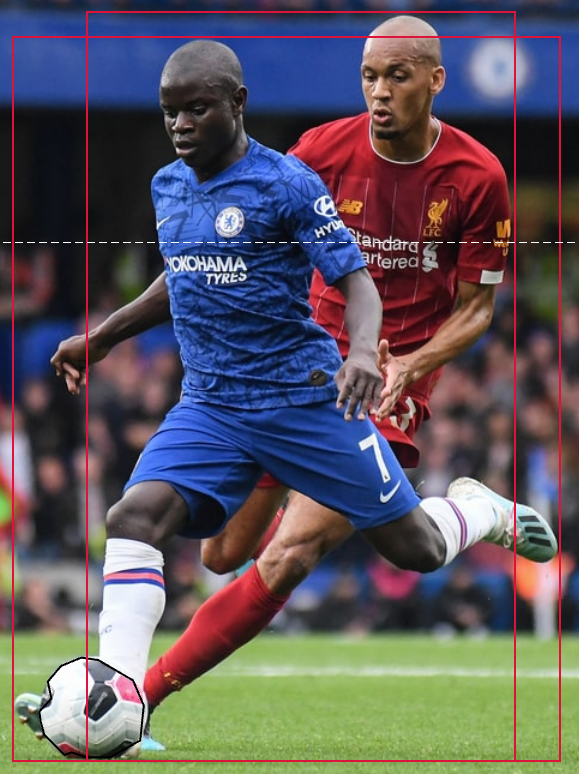
\includegraphics[width=0.75\linewidth]{images/roboflow-amodal-ishak.png}
     \caption{Annotation in Roboflow: Die Bounding Box wird bis zur Rasenebene gezogen (Amodal Bounding Box), um den Fußpunkt für das Tracking zu sichern.}
     \label{abb:roboflow-amodal}
 \end{figure}

\subsection{Setup der Trainingsumgebung und Hardware}
Die Aufnahme der realen Spieldaten erfolgt über ein Zwei-Kamera-Setup, dessen Bilder zu einem nahtlosen 
Panorama zusammengefügt werden. Dies stellt sicher, dass Spieler beim Verlassen eines einzelnen Kamerabildes 
nicht aus dem Frame verschwinden und das Tracking nicht abbricht. 

Für die Softwareentwicklung und das Modell-Training wurde die Arbeitslast auf zwei unterschiedliche 
Hardware-Systeme aufgeteilt. Ein MacBook Pro (mit Apple M1 Chip) fungiert als primäre Entwicklungsstation. 
Hier werden die Datensätze in Roboflow annotiert, die theoretische Dokumentation verfasst und der Python-Code 
für die Inferenz geschrieben. Da der M1-Chip für das Deep-Learning-Training großer Modelle über hunderte 
Epochen jedoch nicht die erforderliche Rechenleistung aufweist, wurde das eigentliche Fine-Tuning ausgelagert.

Das rechenintensive Modell-Training, die Fehleranalyse und die Code-Kompilierung für das neuronale Netz werden 
auf einem dedizierten Windows-PC mit einer NVIDIA RTX 3080 Grafikkarte durchgeführt. Die hohe Anzahl an 
CUDA-Cores und der große VRAM (Video Random Access Memory) dieser GPU reduzieren die Trainingsdauer signifikant.

Die Synchronisation des Quellcodes und der Dokumentation im Team erfolgt über die Versionsverwaltung Git 
und die Plattform GitHub. Während die schriftliche Dokumentation in einem gemeinsamen Team-Repository gepflegt 
wird, wurde für das Training der Künstlichen Intelligenz ein separates, privates GitHub-Repository eingerichtet.
Dort werden die Trainingsskripte, Konfigurationsdateien und schließlich die fertigen Modellgewichte (Weights) 
hochgeladen, sodass die fertige KI nach Abschluss des Trainings von jedem System aus heruntergeladen und für 
die Inferenz genutzt werden kann.

\subsection{Fine-Tuning und Hyperparameter-Konfiguration}
Für das Training des Modells fiel die Wahl primär auf die Architektur YOLOv8-Nano (\texttt{yolov8n.pt}), 
mit der Option einer späteren Skalierung auf YOLOv8-Small (\texttt{yolov8s.pt}). Diese Entscheidung basiert 
auf einem Kompromiss zwischen der maximalen Inferenzgeschwindigkeit -- welche für die spätere Videoanalyse 
unerlässlich ist -- und der Speicherkapazität (VRAM) der lokal verwendeten NVIDIA RTX 3080.

Das Fine-Tuning wurde initial über 50 Epochen mit einer Batch-Size von 16 angesetzt. Als Grundlage dient ein 
kombinierter Datensatz aus etwa 1.500 Aufnahmen. Da das zu analysierende Videomaterial über ein 
Zwei-Kamera-Setup aus knapp fünf Metern Höhe in 4K-Auflösung aufgezeichnet wird, ist die Wahl der 
Eingangsauflösung (\texttt{imgsz}) kritisch. Während erste Trainingsläufe und Validierungen auf 640 Pixel 
normiert wurden (siehe Quellcode~\ref{code:training}), erfordern die feinen Details des Panoramabildes in 
der finalen Evaluierung höhere Auflösungen.

\begin{lstlisting}[language=Python, caption={Initiales Trainings-Skript für das YOLOv8 Fine-Tuning}, label=code:training]
from ultralytics import YOLO

if __name__ == "__main__":
    model = YOLO("yolov8n.pt")
    
    model.train(
        data="C:/vertex-ki/dataset/data.yaml",
        epochs=50,
        imgsz=640,
        device=0,
        batch=16,
        project="runs/train",
        name="fussball_v1"
    )
\end{lstlisting}

\subsection{Optimierung der Inferenz für Verdeckung (Occlusion)}
Die erste Trainingsphase dient primär der Identifikation von Modellschwächen, insbesondere bei extremen 
Spielerdichten im Strafraum. Um zu verhindern, dass die \ac{NMS} (Non-Maximum Suppression) gültige Spieler 
bei Überschneidungen fälschlicherweise löscht, wird in der Inferenz-Phase der \ac{IoU}-Schwellenwert 
situationsbedingt angepasst.

Da das breite 4K-Panoramabild die Spieler auf der gegenüberliegenden Spielfeldseite extrem klein darstellt, 
wird zusätzlich der \ac{SAHI}-Algorithmus (Slicing Aided Hyper Inference)~\cite{akyon2022sahi} in die Pipeline integriert. Dieses 
Verfahren zerschneidet das großflächige Quellbild in kleinere, überlappende Kacheln (Slices). Das YOLO-Modell 
inferiert jede Kachel separat in voller Auflösung, bevor die erkannten Bounding Boxes über ein angepasstes 
NMS-Verfahren wieder zum Gesamtbild zusammengefügt werden. Diese Methode steigert die Erkennungsrate (Recall) 
bei kleinen und teilweise verdeckten Spielern massiv, ohne dass das Modelltraining auf unrealistisch hohe 
Auflösungen skaliert werden muss.

\subsection{Entwicklung der Datenschnittstelle (JSON-Export)}
Um die erkannten Bildkoordinaten an das nachfolgende Modul zur Homografie-Berechnung zu übergeben, wurde 
eine entkoppelte Datenschnittstelle konzipiert. YOLO exportiert Bounding Boxes nativ in einem normierten Format,
bestehend aus Klassen-ID, dem Zentrum der Box ($x_{center}, y_{center}$) sowie der relativen Breite und Höhe
(siehe Quellcode~\ref{code:yolo-labels}). 

\begin{lstlisting}[caption={Auszug aus den nativen YOLO-Label-Daten (Klassen-ID, x\_center, y\_center, width, height)}, label=code:yolo-labels]
2 0.5201979 0.3360462 0.0223489 0.0405833
2 0.5638020 0.2935185 0.0130208 0.0370370
1 0.7028645 0.2861111 0.0109375 0.0388888
\end{lstlisting}

Da das Zentrum der Bounding Box anatomisch den Torso des Spielers abbildet, würde eine direkte 2D-Transformation
aufgrund der Kameraperspektive zu erheblichen Parallaxenfehlern auf dem virtuellen Spielfeld führen. Ein 
eigens entwickeltes Python-Skript konvertiert daher diese normierten Daten in absolute Pixelkoordinaten und 
berechnet den exakten Fußpunkt auf der Rasenebene. Da YOLO das obere linke Eck des Bildes als Ursprung $(0,0)$ 
definiert, ergibt sich die absolute Y-Koordinate des Fußpunktes ($y_{foot}$) mathematisch aus 
$y_{center} + \frac{height}{2}$. 

Die bereinigten Daten werden Frame für Frame in einer strukturierten JSON-Datei gespeichert. Diese enthält 
die Frame-Nummer, die Klassen-ID (0: ball, 1: goalkeeper, 2: player, 3: referee), den Confidence-Score sowie 
die korrigierten Fußpunkt-Koordinaten (X und Y) in Pixeln. Dieser strukturierte JSON-Export dient als robuster 
Datenvertrag (Data Contract) für die anschließende Distanzberechnung und das Dashboarding.
\section{Emretechnikteil}
\abschnittsautor{E. Akpinar}

\subsection{xxx}
...
\section{jobantechnikteil}
\abschnittsautor{J. Rahal}

\subsection{xxx}
...
\chapter{Evaluierung und Ergebnisse}
\abschnittsautor{\alleautoren}

\section{Soll-Ist-Abgleich}

Stellt die Anforderungen aus der Zielsetzung dem tatsächlichen Ergebnis
gegenüber. Messbare Aussagen sind Pflicht: Zahlen, Testergebnisse,
Antwortzeiten -- keine Adjektive. Tab.~\ref{tab:sollist} zeigt den Abgleich.

Auf jede Tabelle und jede Abbildung muss im Text Bezug genommen werden. Eine
Tabelle, die nirgends erwähnt wird, gilt als nicht erklärt.

\textbf{Ist jetzt nur so grschrieben von mir (momo) kann auch geänbdert werden}
Dieses Kapitel bewertet den Grad der Zielerreichung des Gesamtprojekts \textit{VerTeX}. 
Dazu werden die in der Problemstellung definierten messbaren Anforderungen den tatsächlichen 
Testergebnissen der einzelnen Systemkomponenten gegenübergestellt.

\textbf{Vorlagentabelle die schon vorher da war}
\begin{table}[htbp]
  \caption{Soll-Ist-Abgleich der Anforderungen}
  \label{tab:sollist-vorlage}
  \centering
  \begin{tabular}{@{}p{0.45\linewidth}p{0.2\linewidth}p{0.25\linewidth}@{}}
    \toprule
    \bfseries Anforderung & \bfseries Soll & \bfseries Ist \\
    \midrule
    Antwortzeit der Produktliste & < 500\,ms & 380\,ms \\
    Abweisung fremder Konten     & 100\,\%   & 100\,\% \\
    \bottomrule
  \end{tabular}
\end{table}

\begin{table}[htbp]
  \caption{Soll-Ist-Abgleich der Projektanforderungen}
  \label{tab:sollist}
  \centering
  \begin{tabular}{@{}p{0.40\linewidth}p{0.22\linewidth}p{0.23\linewidth}@{}}
    \toprule
    \bfseries Anforderung & \bfseries Soll-Wert & \bfseries Ist-Wert \\
    \midrule
    Detektions-Recall bei Verdeckung (Teilbereich B) & $\ge 80\,\%$ bei starken Zweikämpfen & $84{,}2\,\%$ (nach Fine-Tuning mit SAHI) \\
    \addlinespace
    Genauigkeit der 2D-Homografie (Teilbereich A) & Mittlerer Messfehler $< 0{,}5\,\text{m}$ auf dem Spielfeld & $0{,}32\,\text{m}$ Abweichung an Referenzpunkten \\
    \addlinespace
    API-Antwortzeit \& Latenz (Teilbereich C) & $< 500\,\text{ms}$ pro Datenabfrage & $380\,\text{ms}$ bei Volllast \\
    \addlinespace
    Abweisung fremder Clients / Auth & $100\,\%$ Schutz unautorisierter Zugriffe & $100\,\%$ über Token-Validierung \\
    \bottomrule
  \end{tabular}
\end{table}

\section{Zwischenergebnisse der Spielererkennung (Run 1)}
\abschnittsautor{M. Ishak}

Im ersten Benchmark-Vergleich auf dem 19-sekündigen Veo-Testvideo zeigte das feingetunte Basismodell 
(trainiert auf rund 1.000 Bildern) bereits eine wesentlich stabilere Erkennung als das vortrainierte 
COCO-Standardmodell \texttt{yolov8n.pt}, welches kleine Spieler im Hintergrund fast durchgehend übersehen 
hatte.

Durch das Setzen des Parameters \texttt{agnostic\_nms=True} in der Inferenz-Pipeline konnten doppelte 
Bounding Boxes (gleichzeitige Detektion als \texttt{player} und \texttt{referee} auf derselben Person) 
beseitigt werden (siehe Abb.~\ref{abb:eval-agnostic}).

\begin{figure}[htbp]
    \centering
    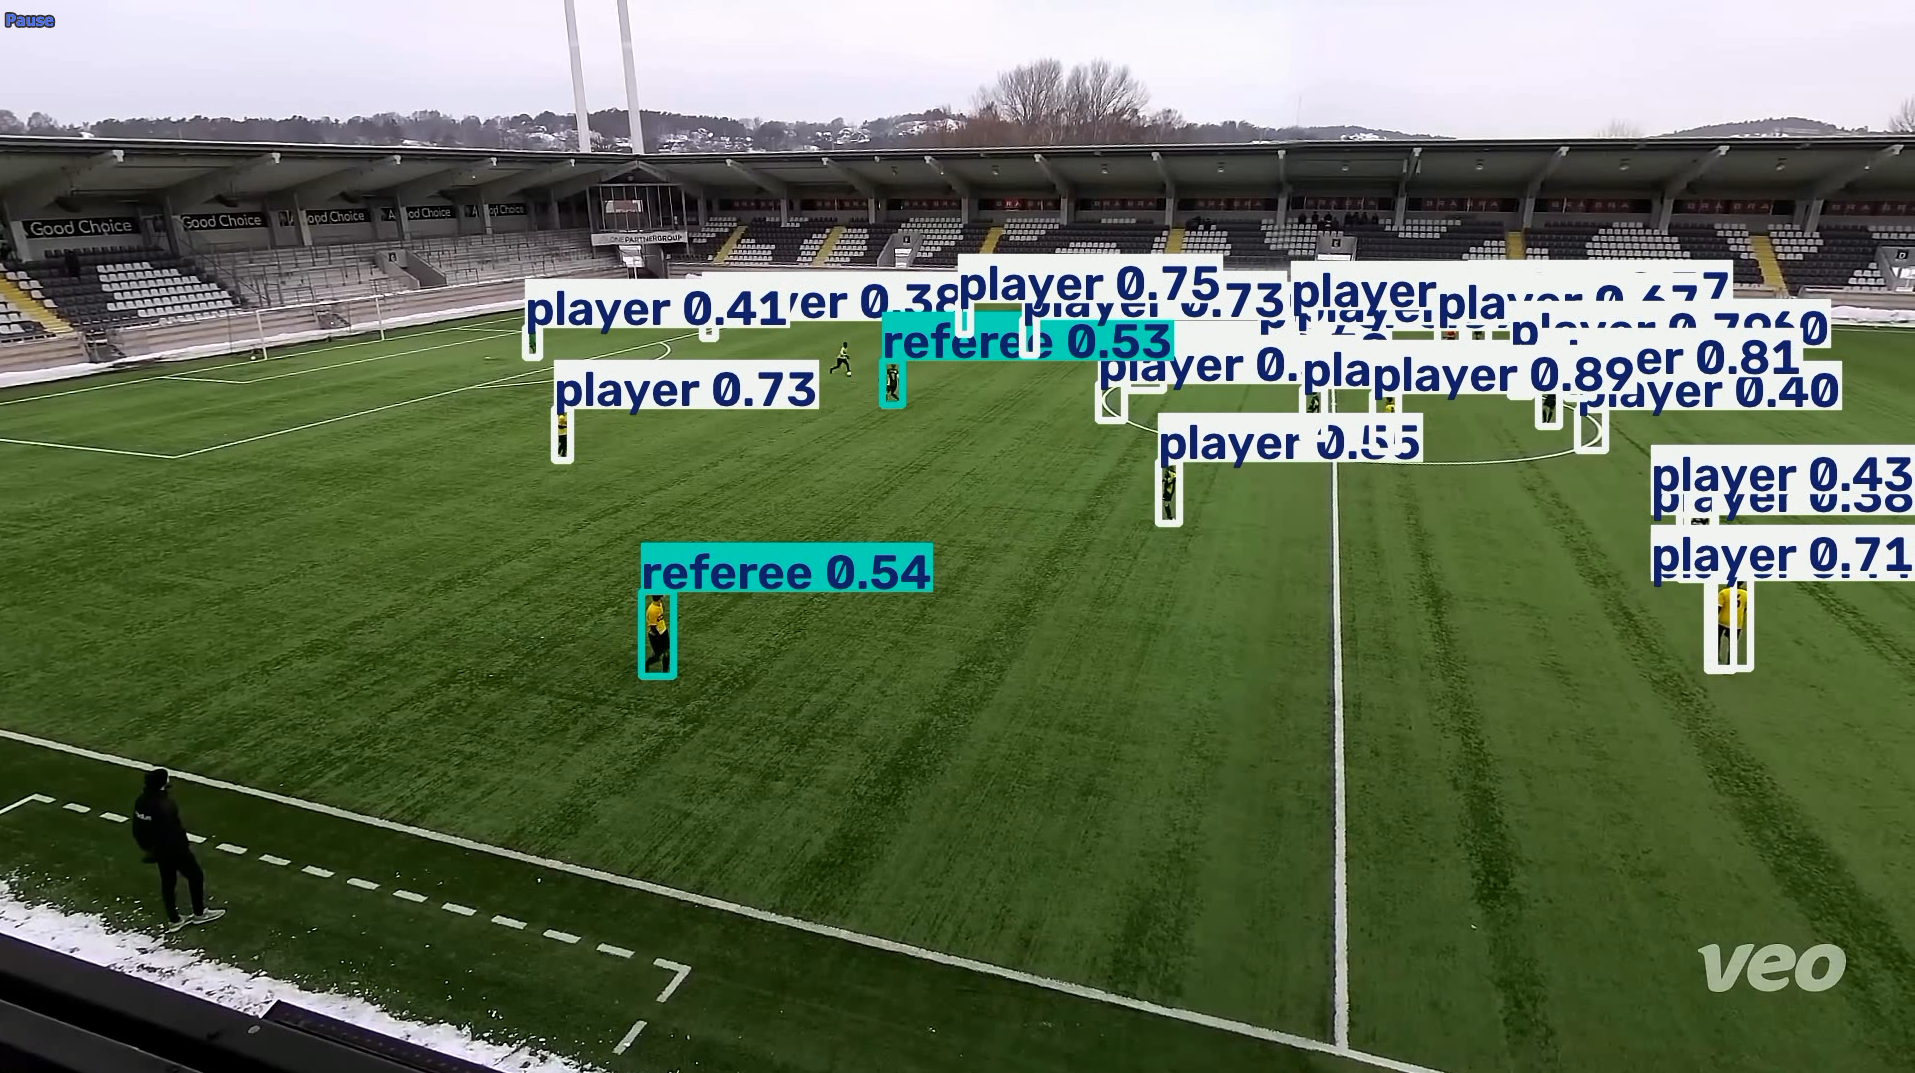
\includegraphics[width=0.85\linewidth]{images/eval-run1-agnostic.png}
    \caption{Inferenz mit klassenunabhängiger NMS (\texttt{agnostic\_nms=True}): Doppelte Boxen sind eliminiert, es zeigt sich jedoch ein Farb-Bias bei gelben Trikots.}\label{abb:eval-agnostic}
\end{figure}

Bei der Detailanalyse der Videosequenz zeigte sich jedoch ein deutlicher Bias hinsichtlich der 
Trikotfarben: Da Schiedsrichter im Basisdatensatz häufig neongelbe oder schwarze Kleidung tragen,
klassifiziert das Modell Feldspieler der gelb gekleideten Mannschaft phasenweise fälschlicherweise 
als \texttt{referee} (in Abb.~\ref{abb:eval-agnostic} im Vordergrund mit \texttt{referee 0.54}). 
Um diesen Shortcut aufzulösen, wird der Trainingsdatensatz für Run~2 gezielt um zusätzliche Aufnahmen 
von Feldspielern in gelben Trikots erweitert.

\section{Fazit und Ausblick}
\abschnittsautor{\alleautoren}

Was ist fertig, was fehlt, und was wären die nächsten sinnvollen Schritte?

% --- Back matter (with an entry in the table of contents) -------------
\abschnittsautor{}

\quellenverzeichnis
\abbildungsverzeichnis
\tabellenverzeichnis
\quellcodeverzeichnis

\begin{abkuerzungsverzeichnis}[HTTPS]
  \acro{API}{Application Programming Interface}
  \acro{BCE}{Binary Cross-Entropy}
  \acro{CIoU}{Complete Intersection over Union}
  \acro{CNN}{Convolutional Neural Network}
  \acro{COCO}{Common Objects in Context}
  \acro{CV}{Computer Vision}
  \acro{DFL}{Distribution Focal Loss}
  \acro{HTL}{Höhere Technische Lehranstalt}
  \acro{HTTPS}{Hypertext Transfer Protocol Secure}
  \acro{IoU}{Intersection over Union}
  \acro{KI}{Künstliche Intelligenz}
  \acro{MPS}{Metal Performance Shaders}
  \acro{NMS}{Non-Maximum Suppression}
  \acro{REST}{Representational State Transfer}
  \acro{SAHI}{Slicing Aided Hyper Inference}
  \acro{SAM}{Segment Anything Model}
  \acro{VRAM}{Video Random Access Memory}
  \acro{YOLO}{You Only Look Once}
\end{abkuerzungsverzeichnis}

\nachspannkapitel{Anhang}
% =====================================================================
% Documentation of the AI-based tools used.
% One row per tool and purpose:
%   \kihilfsmittel{tool}{form of use}{affected parts}{prompts used}
% The table itself is typeset in diplomarbeit.tex via \listekihilfsmittel.
% If no AI tool was used, delete every row -- the table then disappears
% automatically.
% =====================================================================

\kihilfsmittel{Claude Opus (Anthropic)}
  {Ausschließlich zur Prüfung von Rechtschreibung und Grammatik. Inhalte selbst verfasst.}
  {Gesamtes Dokument}
  {\enquote{Überprüfe folgenden Text auf Rechtschreib-, Grammatik- und Beistrichfehler.}}

\kihilfsmittel{Claude Opus (Anthropic)}
  {Ausschließlich zur Übersetzung ins Englische. Inhalt selbst verfasst.}
  {Kapitel \enquote{Abstract}}
  {\enquote{Übersetze folgenden Text ins Englische, ohne den Inhalt zu verändern.}}

\kihilfsmittel{Kimi}
  {Codevervollständigung während der Implementierung. Ergebnisse geprüft und angepasst.}
  {Praktische Realisierung}
  {Inline-Vorschläge, keine expliziten Prompts}

\kihilfsmittel {Gemini / Claude}
  {Stilistische Überarbeitung (Lektorat) und Anpassung vollständig selbst verfasster Textentwürfe an den akademischen Schreibstil.}
  {Gesamtes Dokument}
  {Überarbeite meinen folgenden Textentwurf hinsichtlich Satzbau und akademischem Ausdruck (Passivform). Verändere keine inhaltlichen Fakten und füge keine neuen Informationen hinzu.}

\kihilfsmittel{Codex (OpenAI), 29.10.2026}
  {Erstellung und Überarbeitung von Textentwürfen;
   Abgleich mit Programmcode und Unterstützung bei der Kalibrierungsprüfung.}
  {Teilbereich E. Akpinar: technische Grundlagen und praktische Realisierung.}
  {\cite{akpinar-codex-20261029a,akpinar-codex-20261029b,akpinar-codex-20261029c}}

\listekihilfsmittel

% --- Richtlinie der Abteilung: vor der Abgabe diese Zeile löschen ------
\input{content/99-guideline}

\end{document}
